\documentclass[12pt]{article}
\usepackage[a4paper, total={7in, 10in}]{geometry}
\usepackage[utf8]{inputenc}
\usepackage{amsmath}
\usepackage{amsfonts}
\usepackage{amssymb}
\usepackage{amsthm}
\usepackage{caption}
\usepackage{subcaption}
\usepackage{xeCJK}
\usepackage{fontspec}
\usepackage{graphicx}
\usepackage{float}
\usepackage{hyperref}
\usepackage{bussproofs}
\usepackage{mathtools}
\usepackage{indentfirst}
\usepackage{xcolor}
\usepackage{listings}
\usepackage{afterpage}
\theoremstyle{definition}
\newtheorem{theorem}{Theorem}[subsection]
\newtheorem{definition}[theorem]{Definition}
\newtheorem{corollary}{Corollary}[theorem]
\newtheorem{lemma}[theorem]{Lemma}
\newtheorem{proposition}[theorem]{Proposition}
\DeclareMathOperator{\trace}{\text{tr}}
\DeclareMathOperator{\diag}{\text{diag}}
\newcommand{\colvec}[2][0.8]{
  \scalebox{#1}{
    \renewcommand{\arraystretch}{.8}
    $\begin{bmatrix}#2\end{bmatrix}$
  }
}

\definecolor{codegreen}{rgb}{0,0.6,0}
\definecolor{codegray}{rgb}{0.5,0.5,0.5}
\definecolor{codepurple}{rgb}{0.58,0,0.82}
\definecolor{backcolour}{rgb}{0.90,0.90,0.90}

\lstdefinestyle{mystyle}{
    backgroundcolor=\color{backcolour},   
    commentstyle=\color{codegreen},
    keywordstyle=\color{magenta},
    numberstyle=\tiny\color{codegray},
    stringstyle=\color{codepurple},
    basicstyle=\ttfamily\footnotesize,
    breakatwhitespace=false,         
    breaklines=true,                 
    captionpos=b,                    
    keepspaces=true,                 
    numbers=left,                    
    numbersep=5pt,                  
    showspaces=false,                
    showstringspaces=false,
    showtabs=false,                  
    tabsize=4
}

\lstset{style=mystyle}
%%%%%%%%%%%%%%%%%%%%%%%%%%%%%%
\setCJKmainfont{AR PL UKai TW}
\renewcommand{\baselinestretch}{1.25}
\setlength{\parindent}{2em}
%%%%%%%%%%%%%%%%%%%%%%%%%%%%%%
\begin{document}
%%%%%%%%%%%%%%%%%%%%%%%%%%%%%%
\title{Visualizing the Gibbs Phenomenon \\
  \large 111-2 Data Science and Computer Programming Final Project}
\author{Hsin-Yen, Chiang}
\maketitle
%%%%%%%%%%%%%%%%%%%%%%%%%%%%%%
\section{Abstract}
This project visualize the Gibbs phenomenon in Fourier analysis using Python with \texttt{numpy} and \texttt{matplotlib} libraries.

\section{Introduction}
Fourier series is often used to represent periodic functions as a sum of sine and cosine functions. It allows us to express complex functions in terms of simpler harmonic components. However, when attempting to approximate a function with jump discontinuities, such as Heaviside step function
\[ H(x) := 
\begin{cases}
    0,\ &x<0\\
    \frac{1}{2},\ &x=0\\
    1,\ & x>0
\end{cases}
\]
or a square wave, the Gibbs phenomenon occurs: the Fourier series "overshoots", and the overshoot of the maxima and minima is about 9 percent of the jump in the function for each.

We consider a function $f:\mathbb{R}\to\mathbb{R}$ defined by
\[ f(x) = 
\begin{cases}
    a,\ &-\pi \leq x < 0 \\
    b,\ &0\leq x\leq \pi
\end{cases}
\]
and suppose $a < b$. Let $s_n(x)$ denote the $n$-th partial sum of the Fourier series. Then the maximum of $s_n$ occurs at $\pi/2n$ and the minimum at $-\pi/2n$ and
\[ \lim_{n\to\infty} s_n\left(\frac{\pi}{2n}\right) = \left(\frac{b-a}{2}\right) \left( \frac{2}{\pi} \int_0^\pi \frac{\sin t}{t}\,dt + 1\right) + b \approx (b-a)(0.089) + b. \]
Similarly,
\[ \lim_{n\to\infty} s_n\left(-\frac{\pi}{2n}\right) = \left(\frac{b-a}{2}\right) \left( -\frac{2}{\pi} \int_0^\pi \frac{\sin t}{t}\,dt + 1\right) + a \approx a - (b-a)(0.089).\]
We see that the overshoot of the maxima and minima are about 9 percent of the jump $b-a$.

\newpage

\section{Result}

We first import the library that we needed.
\begin{lstlisting}[language=Python]
    import numpy as np
    import matplotlib.pyplot as plt
\end{lstlisting}

Then we a graph with the square wave function in black and the $n$-partial sum of its Fourier series in blue.
\begin{lstlisting}[language=Python]
    amplitude = 1.0
    frequency = 1.0
    duration = 2.0
    sampling_rate = 100000
    n = 20

    t = np.linspace(0, duration, int(sampling_rate * duration), endpoint=False)
    square_wave = amplitude * np.sign(np.sin(2 * np.pi * frequency * t))

    partial_sum = np.zeros_like(t)
    for k in range(1, n+1):
        partial_sum += (4 / (np.pi * (2*k-1))) * np.sin((2 * np.pi * (2*k-1) * frequency * t))

    plt.plot(t, square_wave, label='Square Wave', color='black')
    plt.plot(t, partial_sum, label=f'{n}-th Partial Sum')
    plt.xlabel('Time (s)')
    plt.ylabel('Amplitude')
    plt.title('Fourier Series Partial Sum')
    plt.ylim(-2, 2)
    plt.legend(loc='lower left')
    plt.grid(True)

    # Find the maximum overshoot point and add a label
    overshoot_index = np.argmax(partial_sum)  # Find the index of the maximum overshoot
    overshoot_time = t[overshoot_index]  # Get the corresponding time value
    overshoot_amplitude = partial_sum[overshoot_index]  # Get the overshoot amplitude
    plt.annotate(f'Overshoot: {overshoot_amplitude:.4f}',
                 xy=(overshoot_time, overshoot_amplitude),
                 xytext=(overshoot_time, overshoot_amplitude + 0.5),
                 arrowprops=dict(facecolor='black', arrowstyle='-|>'),
                 bbox=dict(boxstyle='square', facecolor='lightgray'))
    plt.show()
\end{lstlisting}

\newpage

The result is the followings:

\begin{figure}[htbp]
    \centering
    \begin{subfigure}[t]{0.45\textwidth}
        \centering
        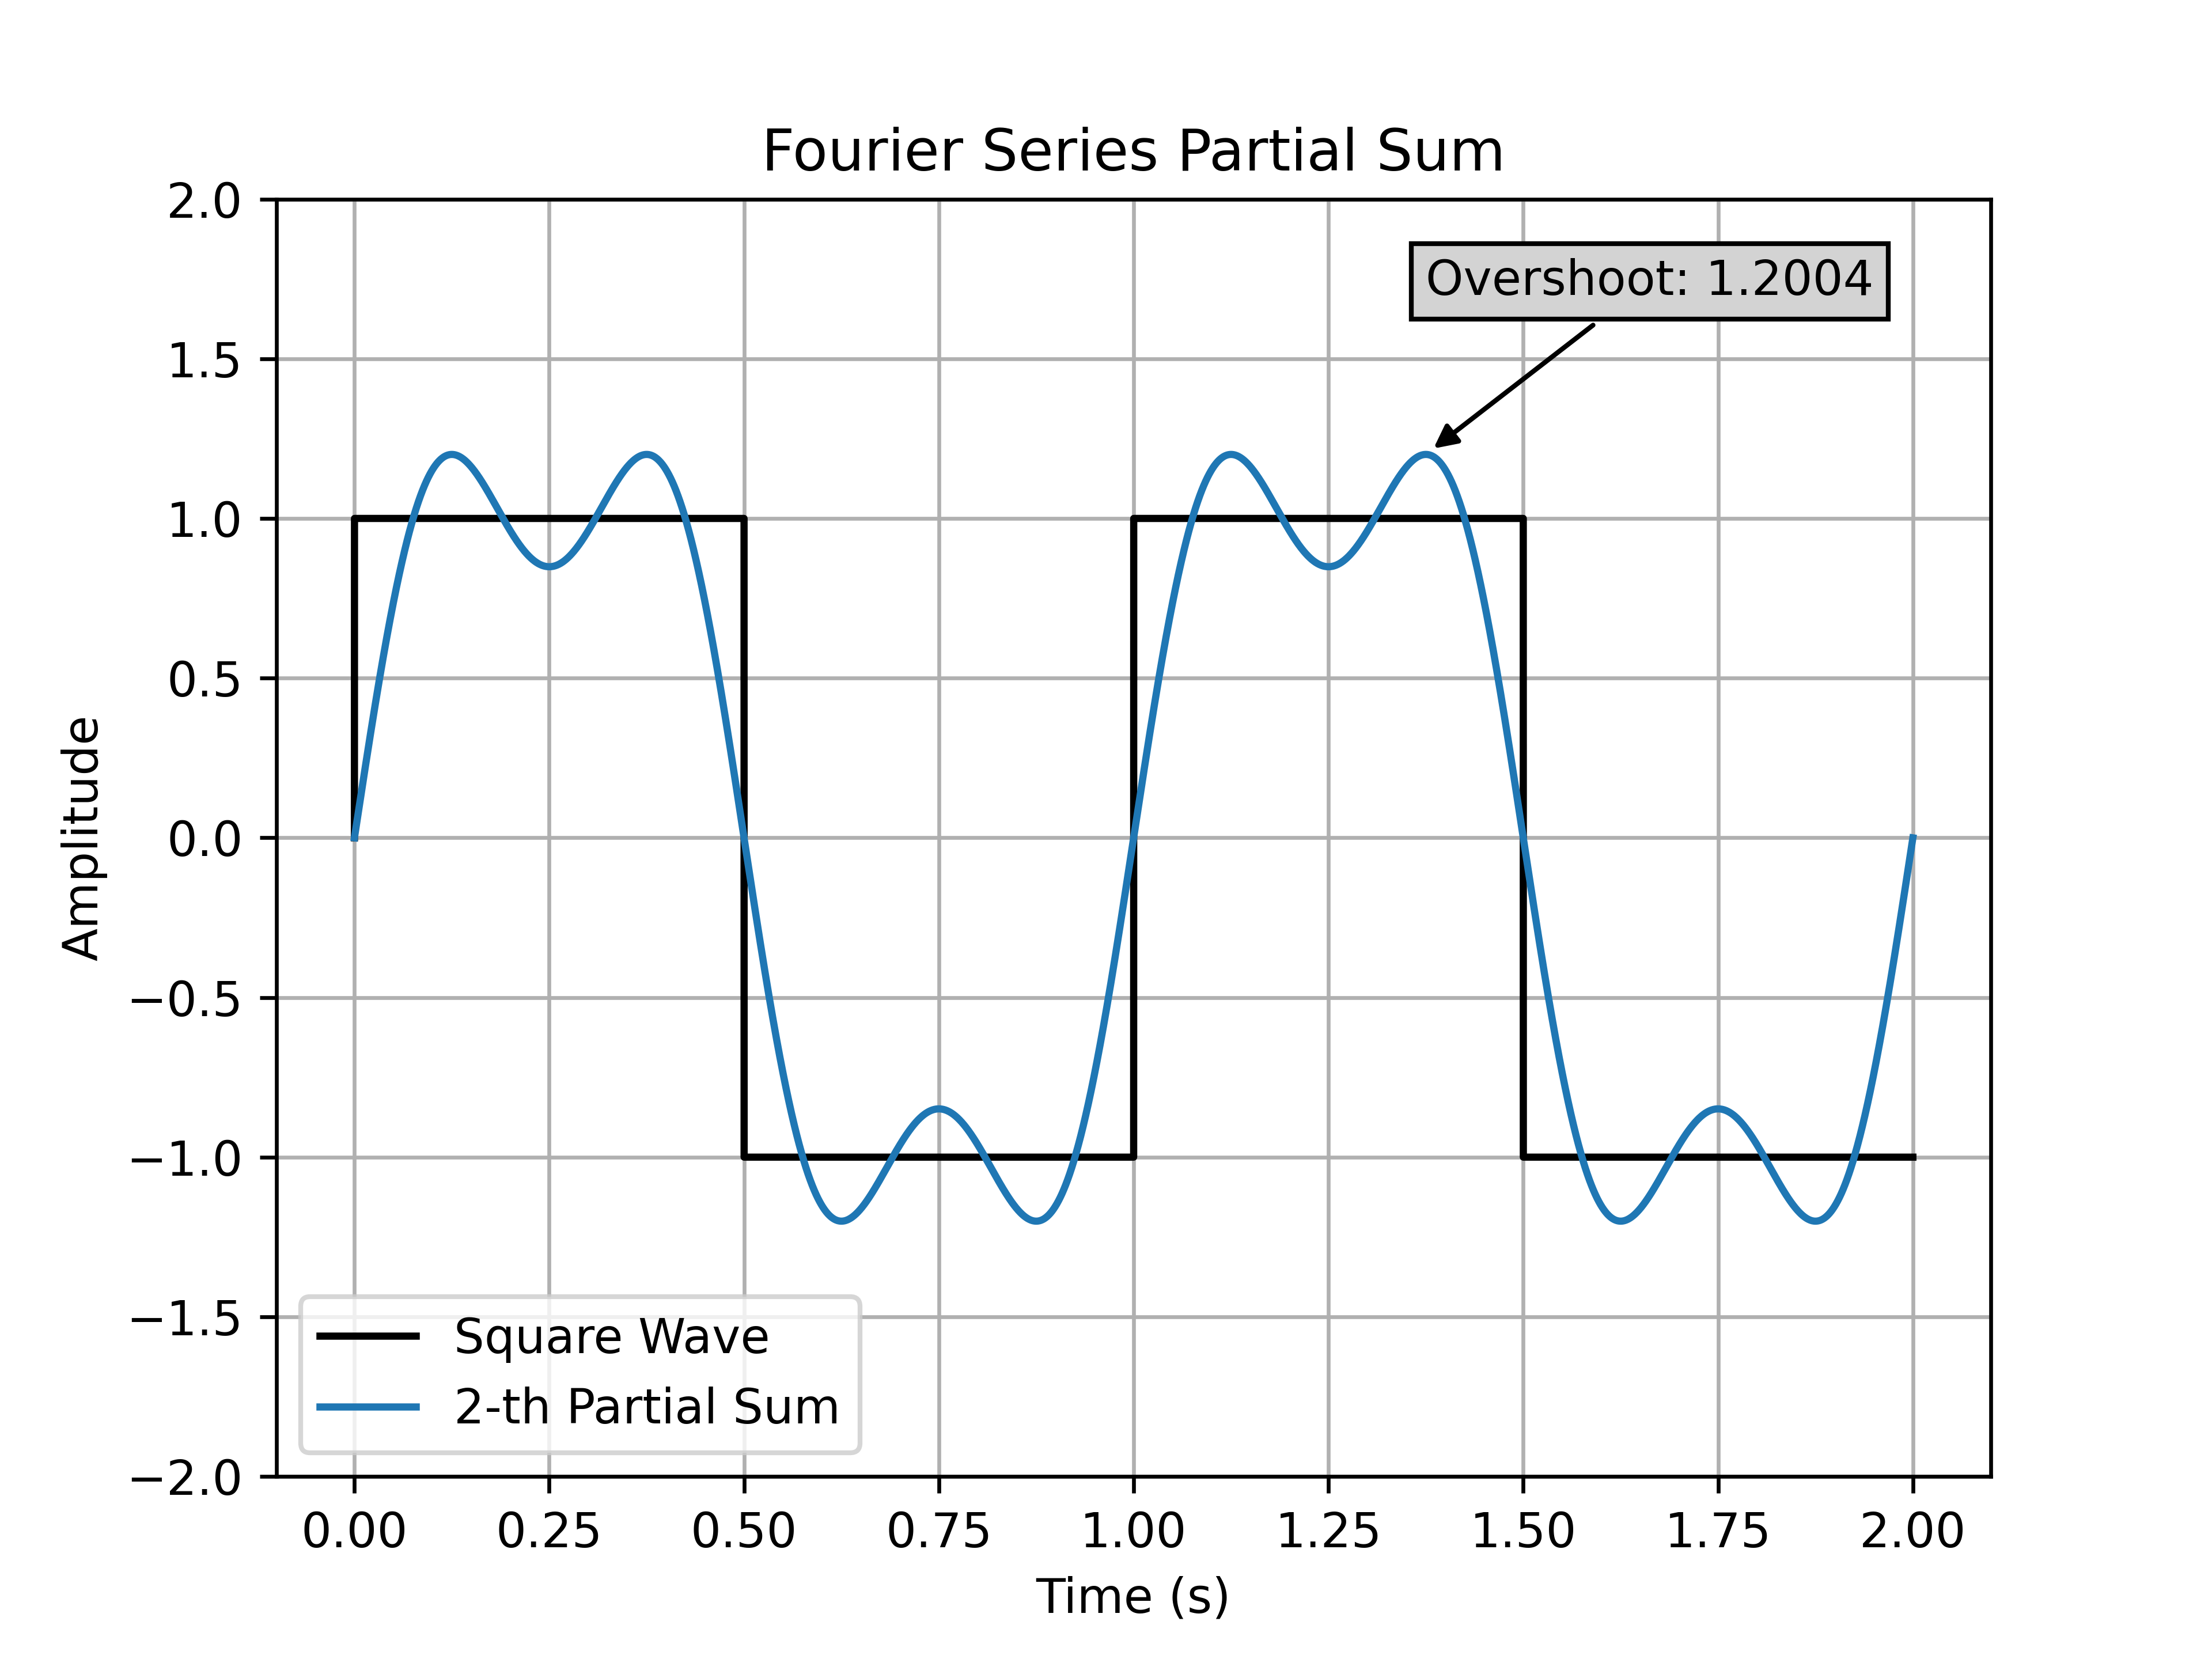
\includegraphics[width=\textwidth]{2-partial.png}
        \caption{2-nd partial sum}
        \label{fig:2-nd partial sum}
    \end{subfigure}
    \quad
    \begin{subfigure}[t]{0.45\textwidth}
        \centering
        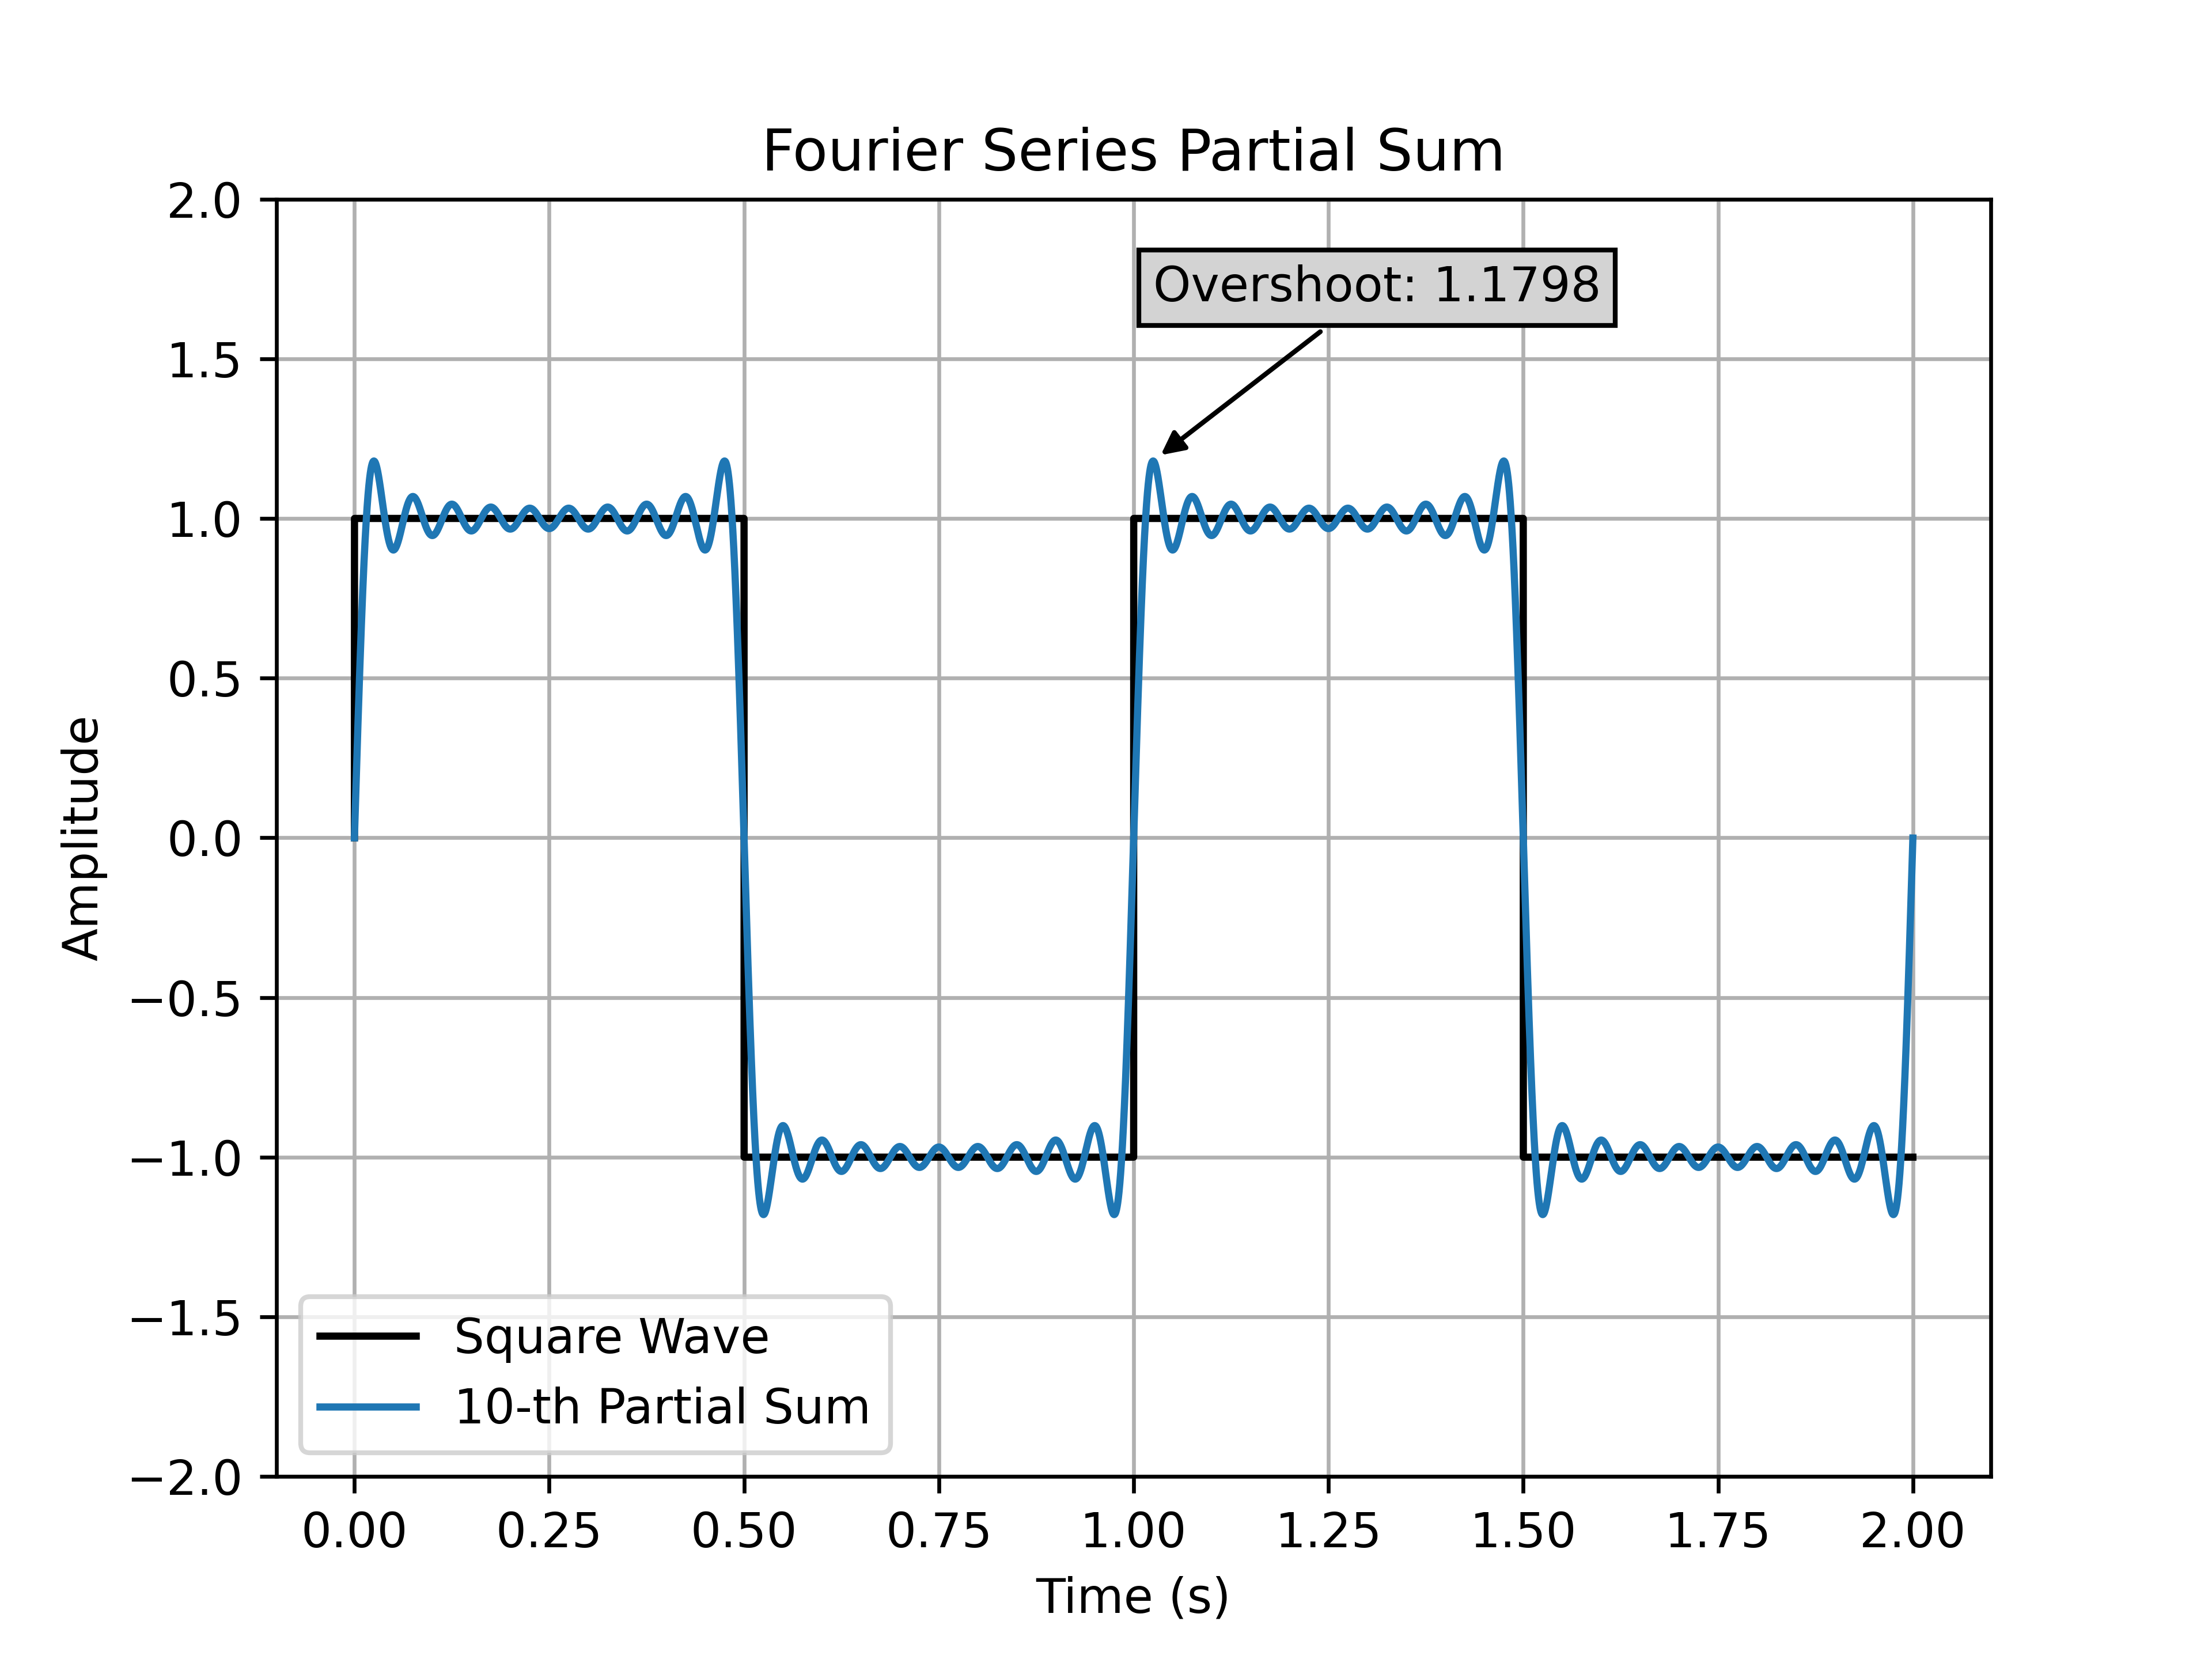
\includegraphics[width=\textwidth]{10-partial.png}
        \caption{10-th partial sum}
        \label{fig:10-th partial sum}
    \end{subfigure}

    \begin{subfigure}[t]{0.45\textwidth}
        \centering
        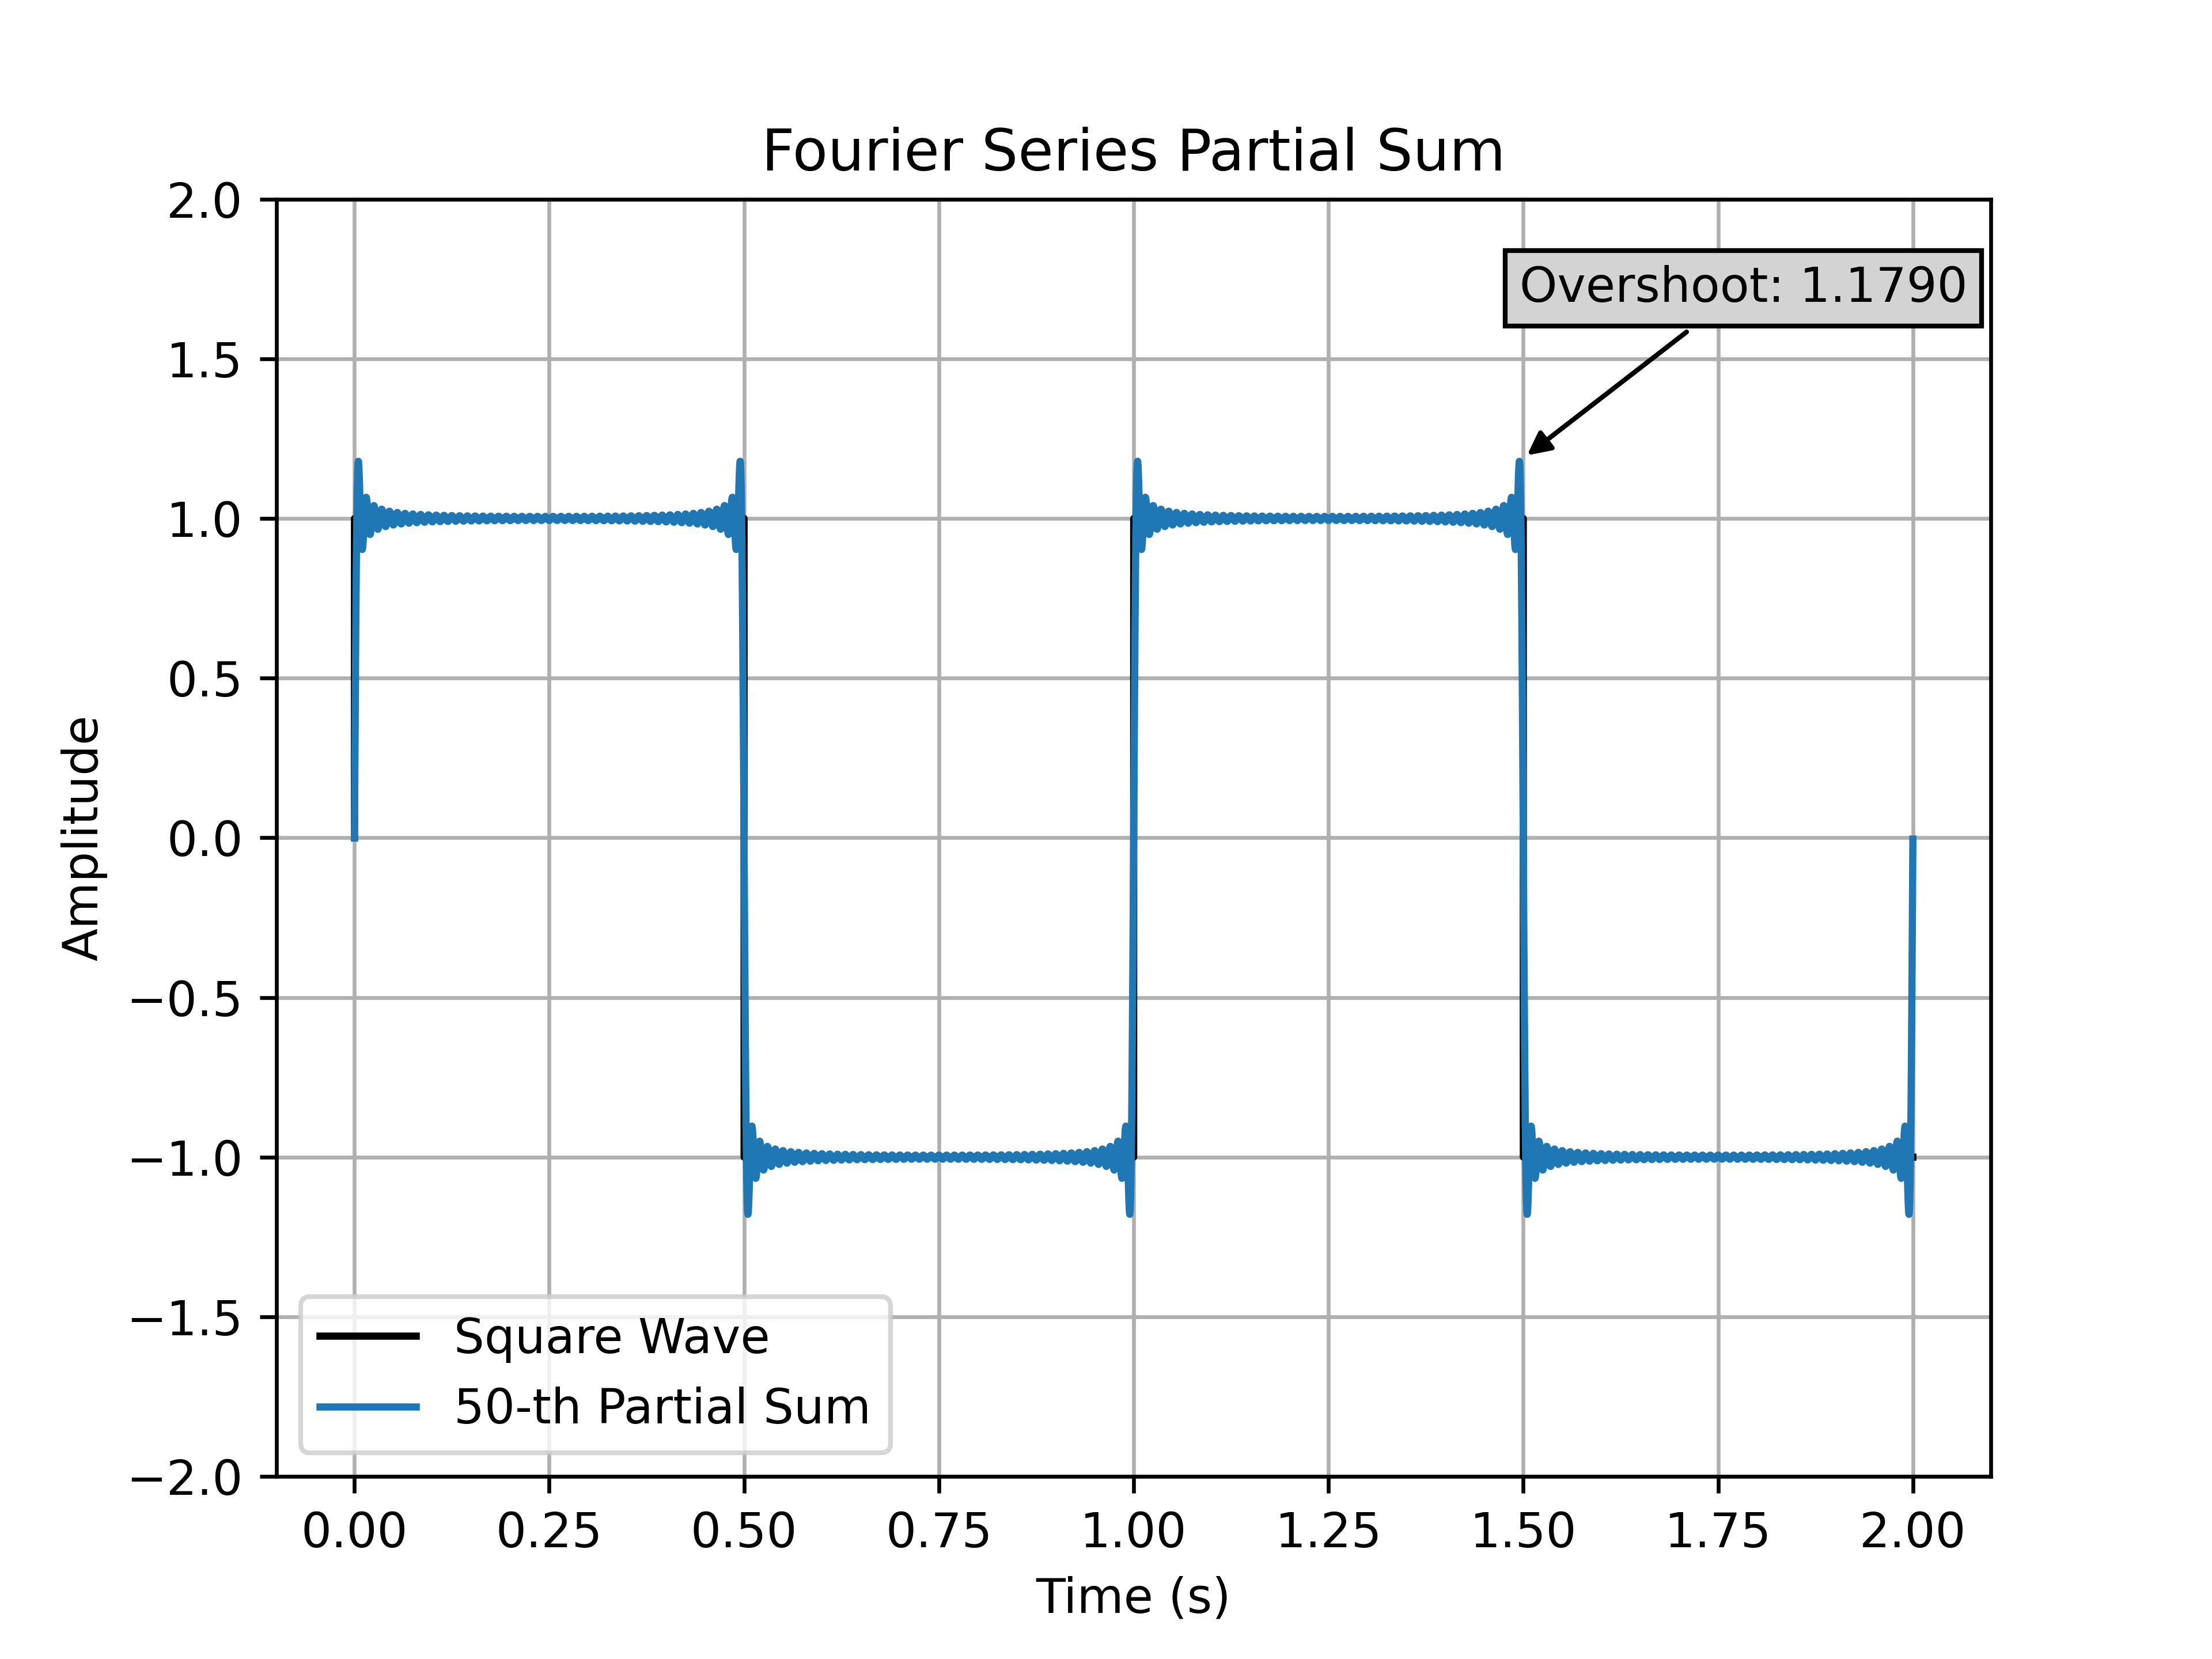
\includegraphics[width=\textwidth]{50-partial.png}
        \caption{50-th partial sum}
        \label{fig:50-th partial sum}
    \end{subfigure}
    \quad
    \begin{subfigure}[t]{0.45\textwidth}
        \centering
        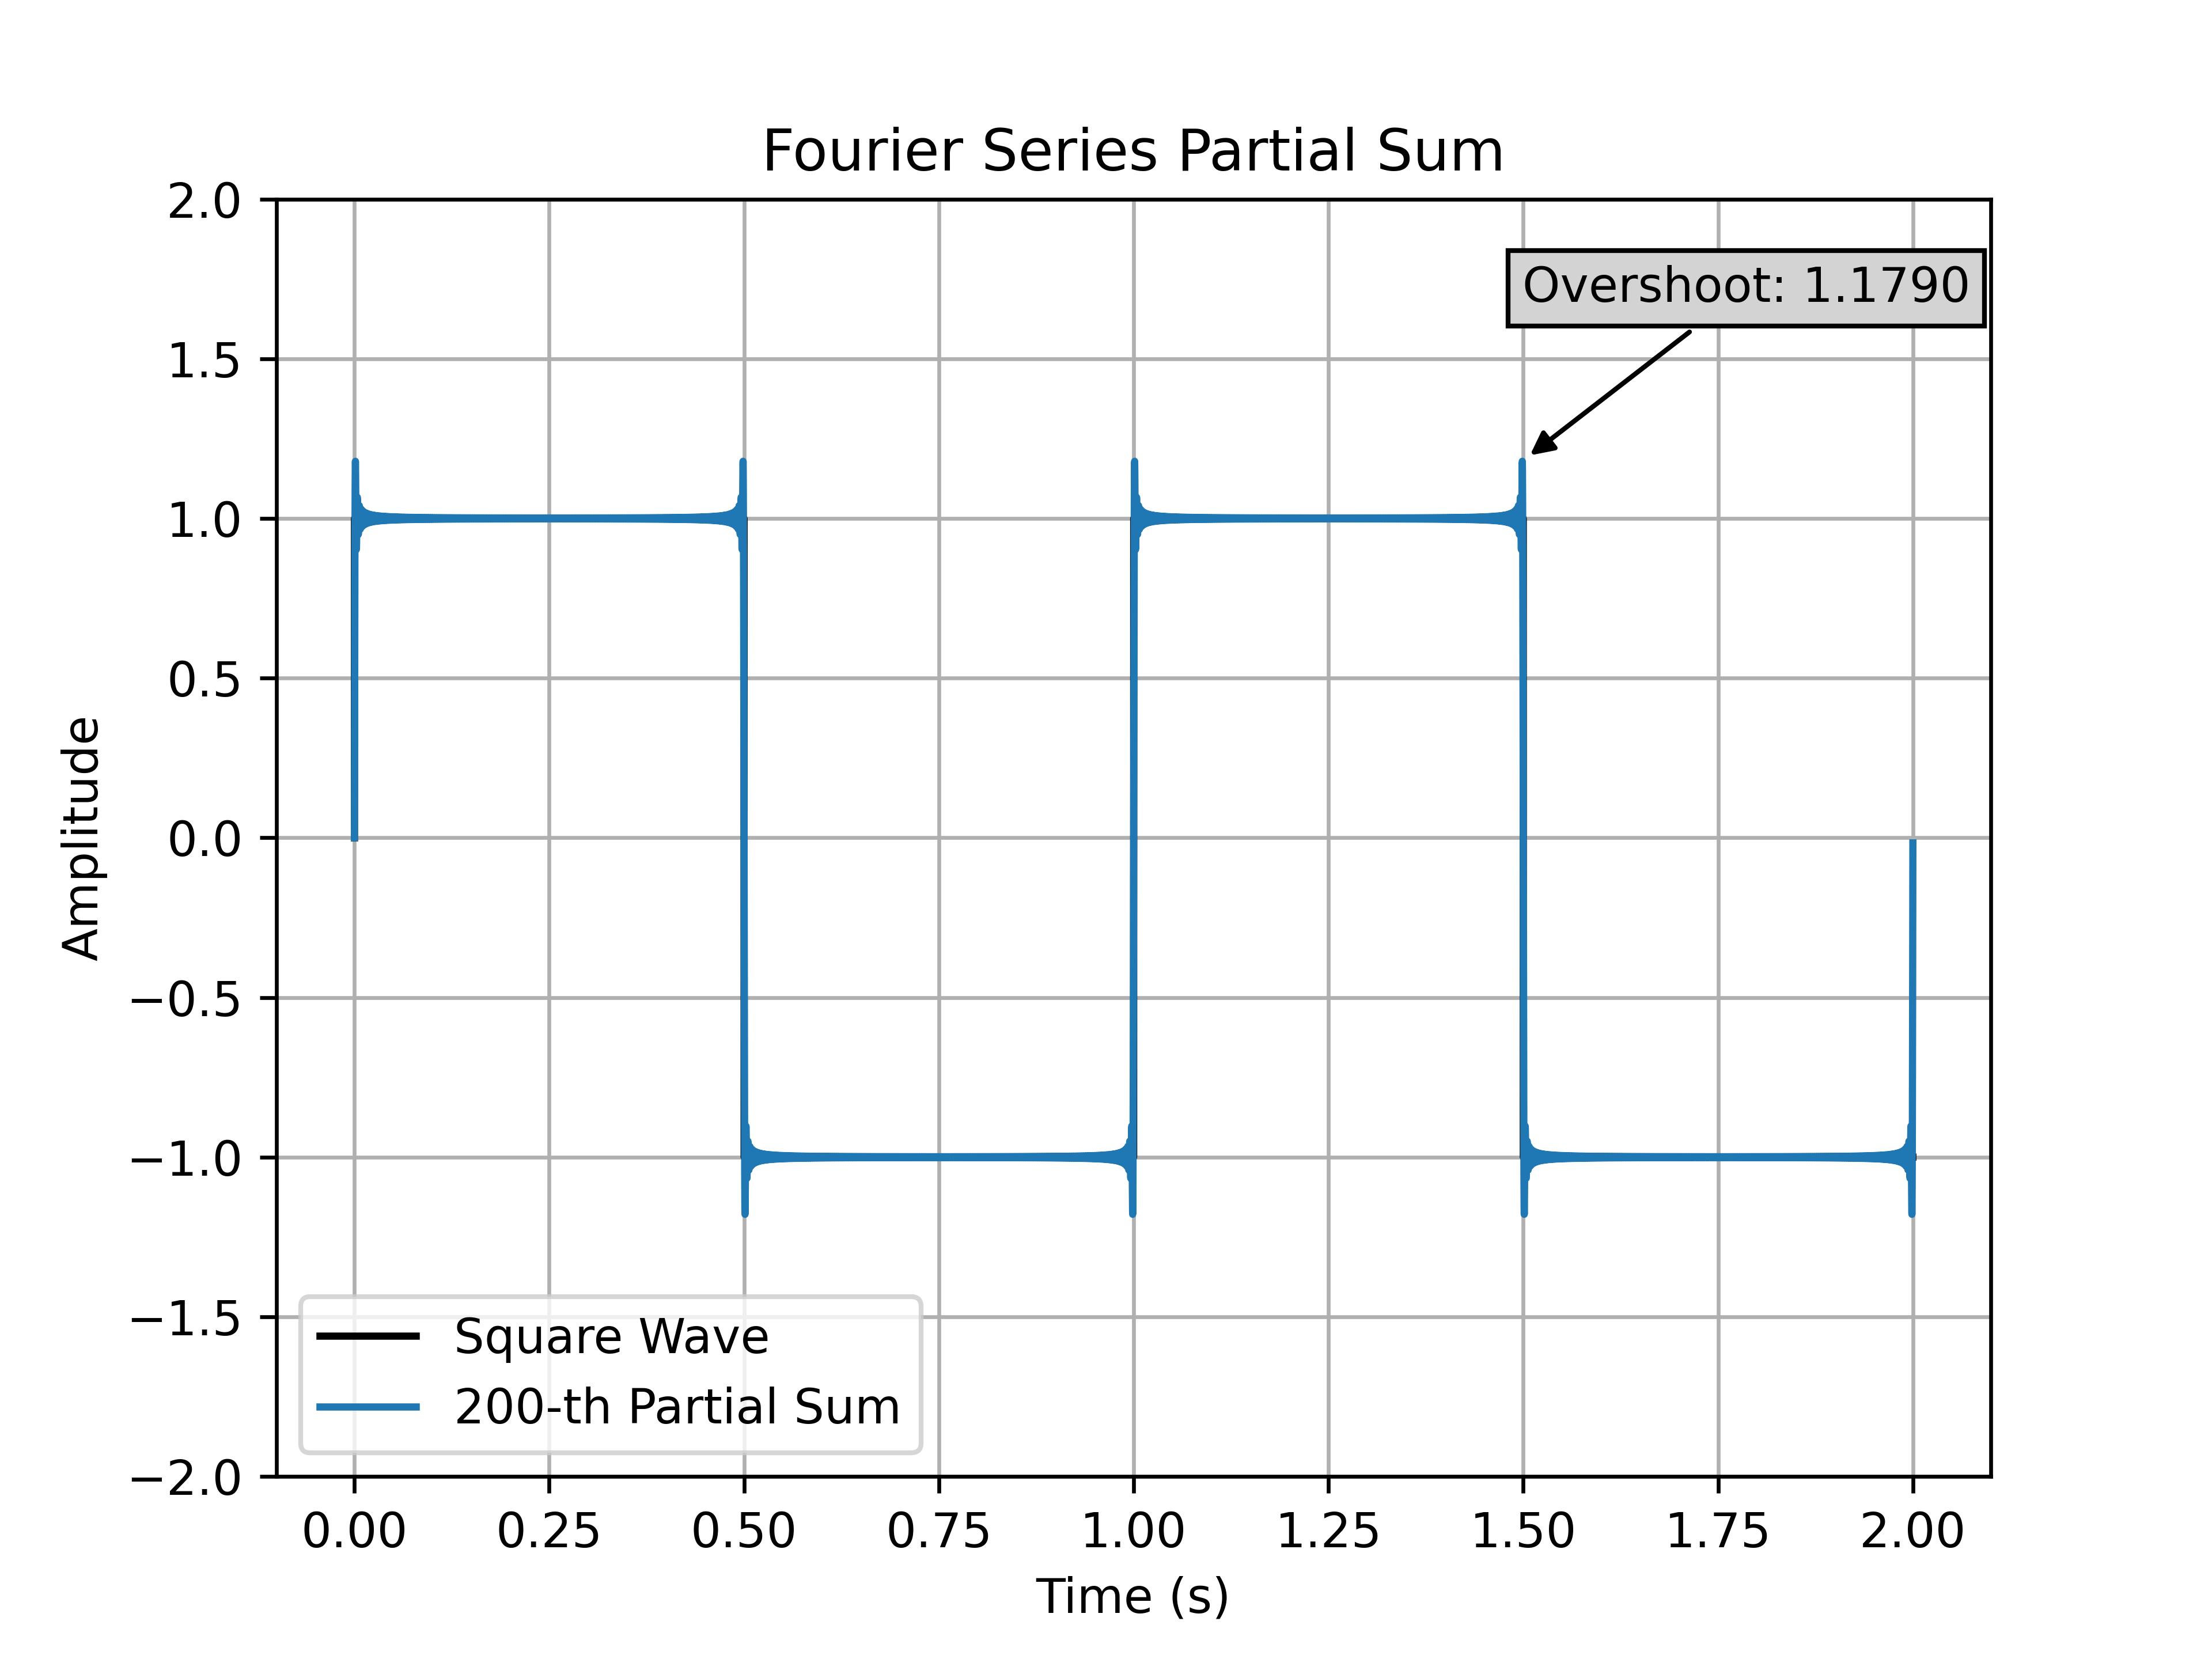
\includegraphics[width=\textwidth]{200-partial.png}
        \caption{200-th partial sum}
        \label{fig:200-th partial sum}
    \end{subfigure}

    \caption{Fourier Series Approaching the Square Wave}
    \label{fig:partial sums}
\end{figure}

In addition, we graph the relation between the value $n$ and the percentage of overshot.
\begin{lstlisting}[language=Python]
    n_values = np.arange(1, 50)  # Specify the range of n values to consider
    overshoot_values = []

    for n in n_values:
        t = np.linspace(0, duration, int(sampling_rate * duration), endpoint=False)
        partial_sum = np.zeros_like(t)
        for k in range(1, n+1):
            partial_sum += (4 / (np.pi * (2*k-1))) * np.sin((2 * np.pi * (2*k-1) * frequency * t))
        # Calculate the overshoot
        overshoot = (np.max(partial_sum) - amplitude) * 50.0
        overshoot_values.append(overshoot)

    plt.plot(n_values, overshoot_values, color='black')
    plt.xlabel('Number of Terms (n)')
    plt.ylabel('Overshoot Percentage (%)')
    plt.title('Relationship between n and Overshoot Percentage')
    plt.grid(True)
    plt.show()
\end{lstlisting}

\afterpage{
    \clearpage
}
    
\begin{figure}[htbp]
    \centering
    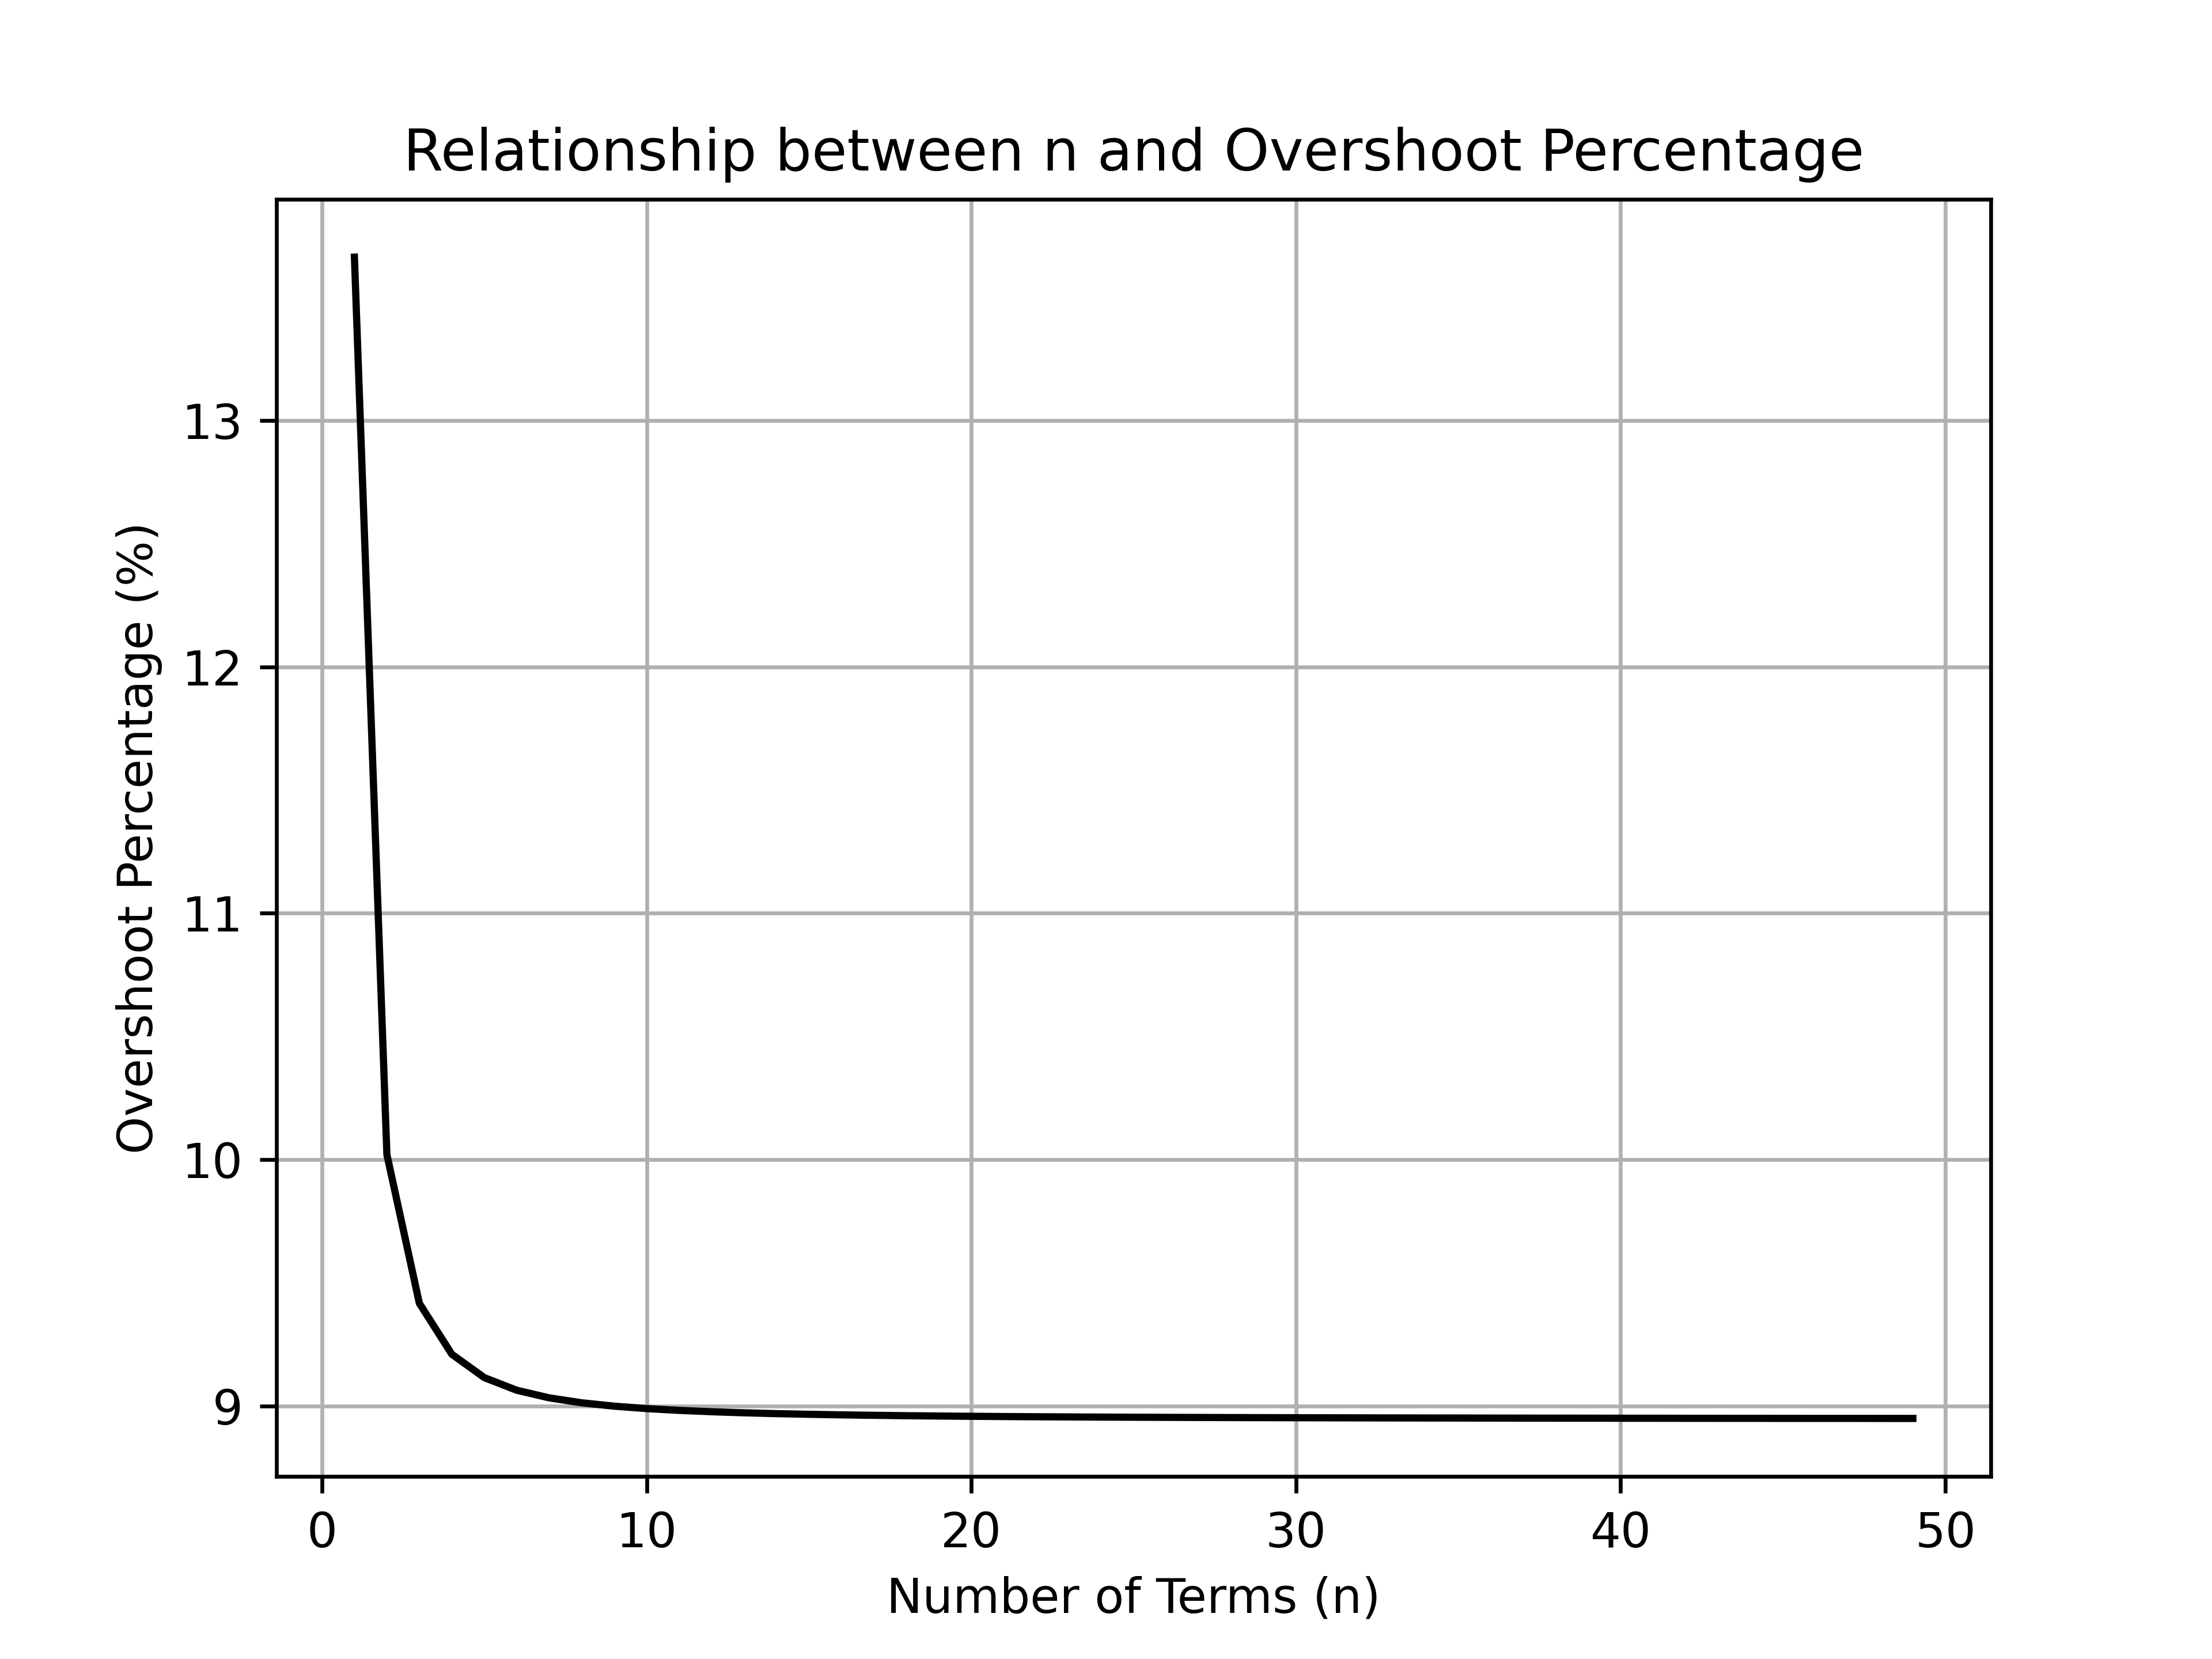
\includegraphics[scale=0.7]{relation.png}
    \caption{Relation Between $n$ and the Overshoot Percentage}
    \label{fig:relation}
\end{figure}

\section{Conclusion}
Through the implementation of the program, we successfully visualized the overshoots at the jump discontinuity of the square wave function. Figure 1 shows that the Fourier series is approaching the function as $n$ becomes larger. On the other hand, Figure 2 provides a visual representation of the approaching of the overshoot percentage to the theory given.

Overall, this visualization may deepen the students' understanding of the Gibbs phenomenon. However, the limit of current program is that an easy way to enter various function with jump discontinuity is not provided.

\begin{thebibliography}{9}
    \bibitem{marsden2008elementary}
    Marsden, J. E. (2008).
    \emph{Elementary Classical Analysis}, 2nd edition.
    W. H. Freeman
\end{thebibliography}

\end{document}